\documentclass[12pt,a4paper]{article}
\usepackage{../lecture-notes/vkCourseML}
\usepackage{lipsum}
\usepackage{indentfirst}
\title{Машинное обучение, ФКН ВШЭ\\Семинар №19}
\author{}
\date{}
\begin{document}
\maketitle

\section{Вывод ALS и HALS}

На лекции была поставлена задача построения модели со скрытыми переменными (latent factor model) для коллаборативной фильтрации:

\[
	\sum_{u,i} (r_{ui} - \langle p_u, q_i \rangle)^2 \to \min_{P,Q}.
\label{LFM}
\]

Напомним, что суммирование ведется по всем парам $(u, i),$ для которых известен рейтинг $r_{ui}$ (и только по ним), а $p_u, q_i$ – латентные представления пользователя~$u$ и товара $i$, соответственно, матрицы $P, Q$ получаются путем записывания по столбцам векторов $p_u, q_i$ соответственно.

\subsection{Alternating Least Squares}

Подход ALS (Alternating Least Squares) решает задачу \eqref{LFM}, попеременно фиксируя матрицы $P$ и $Q$, — оказывается, что, зафиксировав одну из матриц, можно выписать аналитическое решение задачи \eqref{LFM} для другой.

\[
	\nabla_{p_u} \bigg[ \sum_{u,i} (r_{ui} - \langle p_u, q_i \rangle)^2 \bigg] = \sum_{i} 2(r_{ui} - \langle p_u, q_i \rangle)q_i = 0
\]
Воспользовавшись тем, что $a^Tbc = cb^Ta$, получим
\[
	\sum_{i} r_{ui}q_i - \sum_i q_i q_i^T p_u = 0.
\]
Тогда окончательно каждый столбец матрицы $P$ можно найти по формуле
\[
	p_u = \bigg( \sum_i q_i q_i^T\bigg)^{-1}\sum_ir_{ui}q_i \;\; \forall u,
\]
аналогично для столбцов матрицы $Q$
\[
	q_i = \bigg( \sum_u p_u p_u^T\bigg)^{-1}\sum_ur_{ui}p_u \;\; \forall i.
\]

Таким образом мы можем решать оптимизационную задачу \eqref{LFM} поочередно фиксируя одну из матриц $P$ или $Q$ и проводя оптимизацию по второй.

\subsection{Hierarchical Alternating Least Squares}

Подход ALS требует вычислений обратных матриц, что накладывает сильные ограничения на размерность скрытых переменных. Альтернативой ALS является подход HALS (Hierarchical Alternating Least Squares), в котором на каждой итерации мы решаем оптимизационную задачу \eqref{LFM} относительно только одной строчки матрицы $P$ или $Q$. Выведем аналитические формулы для $k$-ой строчки матрицы $P$.
\[
	\frac{\partial}{\partial P_{ku}} \bigg[ \sum_{u',i} (r_{u'i} - \langle p_{u'}, q_i \rangle)^2 \bigg] = \sum_{i} 2(r_{ui} - \langle p_u, q_i \rangle)Q_{ki} = 0
\]
\[
	\sum_{i} (r_{ui} - \sum_{s\neq k} P_{su} Q_{si} )Q_{ki} - P_{ku}\sum_i Q_{ki}^2 = 0
\]
\[
	P_{ku} = \frac{\sum_{i} (r_{ui} - \sum_{s\neq k} P_{su} Q_{si} )Q_{ki}}{\sum_i Q_{ki}^2}
\]
%Если обозначить $p^k$ как строчку матрицы $P$, то в векторном виде формула запишется следующим образом:
%\[
%	p^{k} = \frac{(R - \sum_{s\neq k} p^{s} q^{sT} )q^{k}}{q^k q^{kT}}.
%\]
%Аналогично для строчки матрицы $Q$,
%\[
%	q^{k} = \frac{(R - \sum_{s\neq k} p^{s} q^{sT} )^Tp^{k}}{p^k p^{kT}}.
%\]
%
%В этих формулах, не смотря на то, что $p^k$ – строчка матрицы $P$, мы оперируем ей как вектор-столбцом. Иначе говоря, $p^k$ – транспонированная $k$-ая строчка матрицы $P$.

\section{Neural Collaborative Filtering}

\begin{figure}[h!]
\centering
\includegraphics[scale=0.3]{ncf.eps}
\caption{Neural Collаborative Filtering}
\label{ncf}
\end{figure}

Нелинейным обобщением матричных разложений является коллаборативная фильтрация с помощью нейронных сетей. Сопоставим каждому пользователю $u$ one-hot encode вектор $\alpha_u$, у которого на $u$-ом месте стоит $1$, а остальные координаты заполнены нулями, аналогично определим вектор $\beta_i$ для товара $i$. В качестве алгоритма классификации (или регрессии, в зависимости от задачи) будем использовать нейросеть, у которой два полносвязных слоя на входе: один соответствует пользователям и принимает на вход вектор $\alpha_u$, а второй соответствует товарам и принимает на вход вектор $\beta_i$. После входных полносвязных слоев соответствующие представления необходимо сконкатенировать и передать в следующие полносвязные слои (см.~рис.~\ref{ncf}). На выходе нейронной сети мы получаем предсказание $\widehat{r}_{ui}$ (на рисунке обозначено как $\widehat{y}_{ui}$), которое сравниваем с истинным ответом для заданной пары $r_{ui}$ (на рисунке обозначен как $y_{ui}$).
\newpage
Несмотря на свою простоту модель обладает рядом важных достоинств:
\begin{itemize}
	\item мы можем легко обобщить модель на случай, когда у нас есть признаки пользователей или товаров, добавив эти признаки к векторам $\alpha_u$ и $\beta_i$ соответственно (также заметим, что добавление признаков в модель позволяет частично решить проблему холодного старта);
	\item в зависимости от размеров выборки и природы данных мы можем адаптировать архитектуру под свои нужды, например, если у нас есть картинки в качестве признаков товаров, мы можем добавить сверточные слои в нашу нейронную сеть и обучать всю модель end-to-end.
\end{itemize}

В этой модели мы по-прежнему можем получить латентные представления пользователей и товаров. На самом деле, латентными представлениями будут столбцы матрицы весов в первых полносвязных слоях (в предположении, что мы умножаем матрицу весов на вектор признаков справа).

\section{Факторизационные машины}

Пусть обучающая выборка представлена матрицей $X \in \mathbb{R}^{\ell \times d}$, где $\ell$ – кол-во объектов, а $d$ – кол-во признаков. В случае решения задачи построения рекомендательной системы объектами, как правило, являются пары пользователь-товар, для которых известны оценки $r_{ui}$ степени заинтересованности пользователя в товаре. При этом признаки могут разбиваться на группы, описывающие различные составляющие информации о паре (см рис. \ref{feature_table}).

\begin{figure}[h!]
\centering
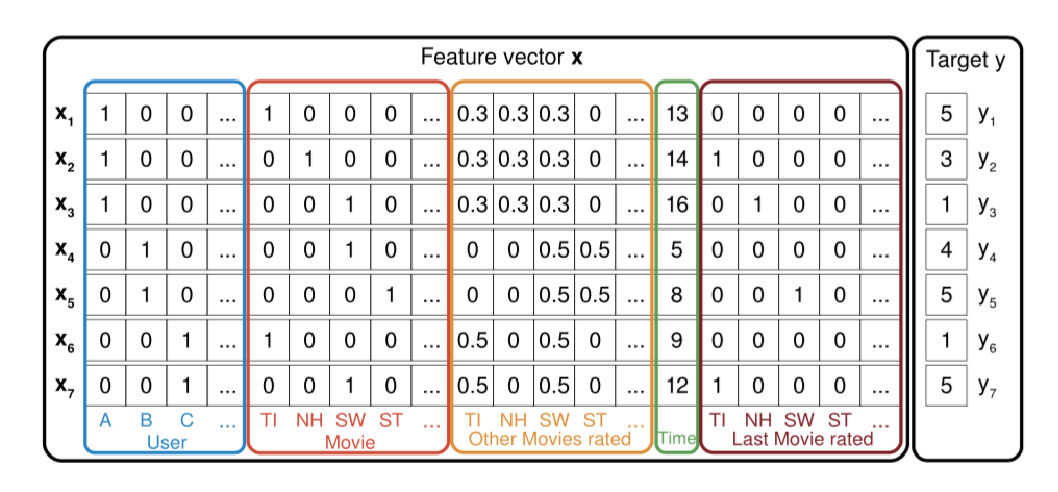
\includegraphics[scale=0.8]{feature_table.eps}
\caption{Представление даннных}
\label{feature_table}
\end{figure}

Факторизационные машины учитывают взаимодействия признаков вплоть до некоторой степени, которая чаще всего равна двум. В этом случае модель будет выглядеть следующим образом:

\begin{equation}
	a(x) = w_0 + \sum_{j=1}^d w_j x_j 
	+ \frac{1}{2} \sum_{j=1}^d\sum_{k=1, \\ k \ne j}^d \langle v_j, v_k \rangle x_j x_k,
\end{equation}

где $w_0, w_1, \dots, w_d \in \mathbb{R}$, $v_1, \dots, v_d \in \mathbb{R}^r$ "--- параметры модели, $x = \left(x_1, \dots, x_d \right)$ "--- признаковое описание объекта. Первое слагаемое соответствует сдвигу, второе слагаемое является линейной моделью, третье слагаемое содержит все попарные взаимодействия $x_j x_k$. В отличие от полиномиальной модели, где каждому попарному взаимодействию $x_j, x_k$ ставится в соответствие индивидуальный вес $w_{jk}$, здесь вес взаимодействия моделируется скалярным произведением двух векторов $\langle v_{j}, v_{k} \rangle$. Иначе можно сказать, что матрица всех весов при слагаемых второго порядка $W$ представима как $W = VV^T,$ где $V = \left[ v_1, \dots, v_d \right]^T$ (т.е. векторы~$v_j$ записаны в строках матрицы~$V$).

Из разложения $W = VV^T$ можно сделать выводы о том, в каких ситуациях применяются факторизационные машины~--- в частности, в случаях, когда количество признаков $d$ очень велико. При $d >> \ell$ обучение полной матрицы весов попарных взаимодействий быстро приводит к переобучению, поэтому в подобных ситуациях параметр $r$ обычно выбирают много меньше $d$.

\subsection{Методы обучения}

Пусть имеется обучающая выборка $X = \{ \left(x_i, \, y_i\right)\}_{i=1}^\ell.$ Параметрами модели являются $\Theta = \left(w_0, w_1, \dots, w_d, v_1, \dots, v_d \right)  = \left(w_0, w_1, \dots, w_d, v_{11}, \dots, v_{dr} \right).$  Задача обучения факторизационной машины формулируется стандартным образом:

\begin{equation}
    Q(a, X) = \sum_{i=1}^\ell L(a(x_i; \Theta), y_i) + \sum_{j = 1}^{|\Theta|} \lambda_j \theta_j^2 \to \min_{\Theta},
\end{equation}

где $\lambda_j$ "--- коэффициент регуляризации параметра $\theta_j, \, L(z, y)$ "--- функция потерь, которая в случае решения задачи регрессии может задаваться как MSE:
\begin{equation*}
	L(z, y) = (z - y)^2,
\end{equation*}
а в случае бинарной классификации (для $y \in \{0, 1\}$) как log-loss:
\begin{equation*}
	L(z, y) = - (1-y)\log(1-z) - y\log z.
\end{equation*}

Второе слагаемое является регуляризатором и может иметь свой коэффициент регуляризации для каждого~$\theta_j$. На практике параметры разбивают на некоторые группы (как на рис. \ref{feature_table}), для каждой из которых выбирают коэффициент регуляризации.
Коэффициент регуляризации для некоторого конкретного параметра~$\theta$ мы будем иногда обозначать как~$\lambda_\theta$.

Существует несколько способов обучения факторизационных машин:
\begin{itemize}
	\item SGD (stochastic gradient descent) "--- оптимизация параметров происходит методом стохастического градиентного спуска по объектам обучающей выборки.
	\item ALS (Alternating Least-Squares) "--- оптимизация параметров происходит попеременно по каждому параметру при фиксированных значениях остальных параметров.
	\item MCMC (Markov Chain Monte Carlo) "--- параметры сэмплируются из апостериорного распределения.
\end{itemize}

\subsubsection{SGD}

Обучение факторизационных машин при помощи SGD осуществуется стандартным образом "--- случайно выбирается один из объектов обучающей выборки, после чего обновляются все параметры модели. Ниже приведён подробный алгоритм обучения.

\begin{algorithmic}
    \REQUIRE{Обучающая выборка $X = \{(x_i, y_i)\}_{i=1}^\ell$, параметры регуляризации $\{\lambda_j\}_{j = 1}^{|\Theta|}$, шаг градиентного спуска~$\eta$, дисперсия инициализации $\sigma$.}
	\ENSURE{Параметры модели $\Theta^* = (w_0^*, \dots, w_d^*, v_1, \dots, v_d).$}
	\vspace{0.5cm}
	\STATE{$w_j := 0, \, j= \overline{0, d}, v_{js} \sim \mathcal{N}(0, \sigma), j = \overline{1, d}, \, s = \overline{1,r};$}
	\REPEAT
	\FOR{$(x_i, \, y_i) \in X$}
    \STATE{$w_0 := w_0 - \eta\bigg(\frac{\partial}{\partial w_0} L(a(x_i; \Theta), y_i) + 2\lambda_{w_0} w_0\bigg)$}
    \FOR{$j\in \{1,\ldots, d\} \text{таких что} x_{ij} \neq 0$}
			\STATE{$w_j := w_j - \eta\bigg(\frac{\partial}{\partial w_j} L(a(x_i; \Theta), y_i) + 2\lambda_{w_j} w_j\bigg)$}
			\FOR{$s \in \{1,\ldots, r\}$}
				\STATE{$v_{js} := v_{js} - \eta\bigg(\frac{\partial}{\partial v_{js}} L(a(x_i; \Theta), y_i) + 2\lambda_{v_{js}} v_{js}\bigg)$}
			\ENDFOR
		\ENDFOR
	\ENDFOR
	\UNTIL{веса не стабилизируются}
\end{algorithmic}

\subsubsection{ALS}
	При обучении факторизационных машин при помощи ALS (или, что в данном случае то же самое, покоординатным спуском) каждый параметр настраивается независимо, т.е. все параметры модели настраиваются поочередно при фиксированных значениях остальных параметров. При этом для каждого параметра можно вывести аналитическую формулу для его оптимального значения на каждом шаге данного метода обучения.

\begin{vkProblem}
	Выразите оптимальное значение некоторого параметра $\theta \in \Theta$ при фиксированных значениях остальных параметров $\Theta \backslash \{\theta \}$ в задаче оптимизации функционала $Q(a, X)$ для задачи регрессии с функционалом MSE.
\end{vkProblem}

\begin{esSolution}
	Заметим, что для любого параметра $\theta \in \{w_0, w_1, \dots, w_d, v_{11}, \dots, v_{dr} \}$ модель $a(x)$ линейна по нему и может быть записана следующим образом:

\begin{align*}
	&a(x) = g_{\theta}(x) + \theta h_{\theta}(x),\\
	&h_{w_0}(x) = 1,\\
	&h_{w_j}(x) = x_j, \, j = \overline{1,d},\\
	&h_{v_{js}}(x) = x_j \sum_{k \ne j} v_{ks} x_k, \, j = \overline{1, d}, \, s = \overline{1, r},
\end{align*}

где функции $g_{\theta}(x)$, $h_{\theta}(x)$ не зависят от значения параметра $\theta$.

Запишем оптимальное значение $\theta^*$ параметра $\theta$ для решаемой оптимизационной задачи:
\begin{align*}
    \theta^* & = \argmin_{\theta} \bigg( \sum_{i=1}^\ell (a(x_i; \theta) - y_i)^2 + \sum_{j = 1}^{|\Theta|}\lambda_j \theta_j^2 \bigg)\\
	& = \argmin_{\theta} \bigg( \sum_{i=1}^\ell (g_{\theta}(x_i) + \theta h_{\theta}(x_i) - y_i)^2 + \sum_{j = 1}{|\Theta|}\lambda_j \theta_j^2 \bigg)\\
	& = \frac{\sum_{i=1}^\ell (y_i - g_{\theta}(x_i))h_{\theta}(x_i)}{\sum_{i=1}^\ell h_{\theta}^2(x_i) + \lambda_{\theta}}.
\end{align*}
\end{esSolution}

Как правило, $g_\theta(x)$ не выражают в явном виде, а используют представление $g_\theta(x) = a(x; \Theta) - \theta h_\theta(x),$ из которого можно вывести формулу обновления параметра $\theta$ при использовании метода ALS:
\begin{align*}
	\theta^* = \frac{\sum_{i=1}^\ell (y_i - g_{\theta}(x_i))h_{\theta}(x_i)}{\sum_{i=1}^\ell h_{\theta}^2(x_i) + \lambda_{\theta}}=
	\frac{\sum_{i=1}^\ell (y_i - a(x_i; \Theta) + a(x_i; \Theta) - g_{\theta}(x_i))h_{\theta}(x_i)}{\sum_{i=1}^\ell h_{\theta}^2(x_i) + \lambda_{\theta}}=\\
	= \frac{\theta \sum_{i=1}^\ell h_{\theta}^2(x_i) + \sum_{i=1}^\ell h_{\theta}(x_i) (y_i - a(x_i; \Theta))}{\sum_{i=1}^\ell h_{\theta}^2(x_i) + \lambda_{\theta}}.
\end{align*}

Это выражение использует текущие значения параметров модели и её прогнозы на объектах обучающей выборки и используется для итеративного обновления каждого параметра $\theta$ при фиксированных значениях остальных параметров при использовании метода ALS для обучения модели.

\subsection{Частные случаи}
\subsubsection{Matrix Factorization}

Пусть решается задача построения рекомендательной системы для множества пользователей $U$ и множества товаров $I$. Воспользуемся факторизационными машинами для решения этой задачи. Естественный путь описания пары $(u,i) \in U\times I$ "--- это бинарный вектор, состоящий из нулей и содержащий ровно две единицы:

\[
  (u,i) = (\underbrace{0,\ldots, 0, 1, 0, \ldots, 0,}_\text{|U|} \underbrace{0,\ldots, 0, 1, 0, \ldots, 0}_\text{|I|}),
\] 

где первая единица соответствует индексу пользователя и стоит на $u$-ом месте, а вторая единица соответствует индексу товара и стоит на $(|U| + i)$-ом месте. Тогда факторизационная машина, обученная на данных, представленных таким образом, будет выглядеть следующим образом:

\begin{equation}
	a(x) = w_0 + w_u + w_{|U|+i} + \langle v_u, v_{|U| + i}\rangle.
\end{equation}

Как видим, данная модель совпадает с моделью в подходе, использующем матричное разложение (со сдвигами $w_u, w_i$), где $v_{u}, v_{|U|+i} \in \mathbb{R}^{r}$ являются векторными представлениями пользователей и товаров соответственно.

\subsubsection{Pairwise Interaction Tensor Factorization}

Допустим, у нас появилась новая информация о товарах~--- помимо множества пользователей $U$ и множества товаров $I$ теперь имеется множество тегов $T$. Естественный путь описания тройки $(u,i,t) \in U\times I$ "--- бинарный вектор, состоящий из нулей и содержащий ровно три единицы:

\[
  (u,i, t) = (\underbrace{0,\ldots, 0, 1, 0, \ldots, 0}_\text{|U|}, \underbrace{0,\ldots, 0, 1, 0, \ldots, 0}_\text{|I|},\underbrace{0,\ldots, 0, 1, 0, \ldots, 0}_\text{|T|}),
\] 

где первая единица соответствует индексу пользователя и стоит на $u$-ом месте, вторая единица соответствует индексу товара и стоит на $(|U|+i)$-ом месте, а третья единица соответствует индексу тега и стоит на $(|U|+|I|+t)$-ом месте. Тогда факторизационная машина, обученная на данных, представленных таким образом, будет выглядеть следующим образом:

\begin{equation}
	a(x) = w_0 + w_u + w_{|U|+i} + w_{|U|+|I|+t} + \langle v_u, v_{|U|+i}\rangle + \langle v_u, v_{|U|+|I|+t}\rangle + \langle v_{|U|+i}, v_{|U|+|I|+t}\rangle.
\end{equation}

Такая модель носит название Pairwise Interaction Tensor Factorization. Разумеется, пример с тегом является очень частный, и вместо тега мы можем использовать любой категориальный признак~(или несколько таких признаков).

\subsubsection{SVD++}

Продолжаем развитие нашей рекомендательной системы. Пусть на этот раз мы столкнулись с~\textit{множествозначным} признаком~-- он может быть равен любому набору категорий из некоторого множества~(например, каждый товар может иметь сразу несколько тегов). Таким образом, объект обучающей выборки представлен двумя категориальными признаками~(пользователь $u$, товар $i$) и множествозначным признаком $l$, который может принимать $m$ ненулевых значений. На Рис. \ref{feature_table} первые три группы признаков соответствуют такому представлению. Как и раньше, опишем такое представление числовым вектором:

\[
  (u,i,l = \{l_1, \ldots l_m \}) = (\underbrace{0,\ldots, 0, 1, 0, \ldots, 0}_\text{|U|}, \underbrace{0,\ldots, 0, 1, 0, \ldots, 0}_\text{|I|},\underbrace{0,\ldots, 1/m, \ldots, 1/m,\ldots, 0}_\text{|L|}),
\] 

Как и в предыдущих пунктах, ненулевые значения полученного вектора являются индикаторами категорий признаков (подмножества категорий в случае множествозначного признака). Модель для факторизационных машин выглядит следующим образом:

\begin{align*}
	a(x) = & w_0 + w_u + w_i + \langle v_{u},  v_{i} \rangle + \frac{1}{m}\sum_{f=1}^k \langle v_{i},  v_{l_{j}} \rangle + \\
	& + \frac{1}{m}\sum_{j=1}^m w_{l_j} + \frac{1}{m}\sum_{j=1}^m \langle v_u, v_{l_j} \rangle + \frac{1}{m^2}\sum_{j=1}^m\sum_{j^\prime}^m \langle v_{l_j}, v_{l_j^{\prime}} \rangle\\
\end{align*}

Первая часть (первая строка уравнения) соответствует модели под названием SVD++. Вторая строчка модели содержит дополнительные взаимодействия между признаками.

\end{document}
